\appendix
\section{Description of the Prompts used in \agentname~Workflow}\label{app:prompt}
\subsection{Prompt for Coder in first round of generation} %(One-shot Baseline Prompt from \textsc{KernelBench})}
We adopt the \emph{One-shot Baseline Prompt} introduced in \textsc{KernelBench} as our initial prompt for first round generation of all the baselines and our method. The full prompt is shown below.

\begin{tcolorbox}[mybox, title={Prompt for Coder in first round of generation}]
You write custom CUDA kernels to replace the PyTorch operators in the given architecture to get speedups.
You have complete freedom to choose the set of operators you want to replace. You may decide to replace
some operators with custom CUDA kernels and leave others unchanged. You may replace multiple operators
with custom implementations, consider operator fusion opportunities (combining multiple operators into a
single kernel, for example, combining \texttt{matmul}+ \texttt{relu}), or algorithmic changes (such as online softmax).
You are only limited by your imagination.

Here is an example to show you the syntax of inline-embedding custom CUDA operators in PyTorch.

\textbf{The example given architecture is:}
\begin{lstlisting}[style=nice, language=Python]
{few_base}
\end{lstlisting}

\textbf{The example new architecture with custom CUDA kernels looks like this:}
\begin{lstlisting}[style=nice, language=Python]
{few_new}
\end{lstlisting}

\textbf{You are given the following architecture:}
\begin{lstlisting}[style=nice, language=Python]
{arch_src}
\end{lstlisting}

Optimize the architecture named \texttt{Model} with custom CUDA operators! Name your optimized output
architecture \texttt{ModelNew}. Output the new code in code blocks. Please generate real code, \emph{NOT}
pseudocode. Make sure the code compiles and is fully functional. Just output the new model code, no other
text, and \textbf{NO} testing code!
\end{tcolorbox}
\lstset{language=python}

\subsection{Prompt for Judge}
In our prompt design for the Judge agent, we place the role specification and output schema in the system prompt. Inspired by ~\citep{agashe2024agentsopenagentic,lei2025infantagentnextmultimodalgeneralistagent,chen2023agentversefacilitatingmultiagentcollaboration}, we design the prompts for correction and optimization, which are shown below.

\begin{tcolorbox}[redbox, title={Prompt for CUDA Kernel Correction}]
\ttfamily

You are a senior CUDA + PyTorch correctness auditor. Your job is to read a PyTorch reference and a CUDA candidate and report \textbf{exactly one} most critical correctness issue in the CUDA code that would cause a behavioral mismatch vs.\ the PyTorch reference. Be terse and precise.

\medskip
\textbf{Rules:}
\begin{itemize}
  \item Return \textbf{one and only one} issue --- the single highest-impact problem.
  \item Prefer semantic/correctness issues over micro-optimizations or style.
  \item If multiple issues exist, pick the one that most changes outputs or gradients.
  \item If nothing clearly wrong is found, say it explicitly.
  \item Keep each field brief; avoid extra commentary, lists, or alternatives.
\end{itemize}

\medskip
\textbf{Output format (JSON):}
\begin{tcolorbox}[colback=white, colframe=gray!50, left=2mm, right=2mm, top=1mm, bottom=1mm]
\footnotesize
\begin{verbatim}
{
  "critical_issue": "<max 20 words>",
  "why_it_matters": "<max 35 words>",
  "minimal_fix_hint": "<max 20 words>"
}
\end{verbatim}
\end{tcolorbox}

\medskip
\textbf{You are given:}

\textbf{ERROR\_LOG:}
\begin{verbatim}
{ERROR_LOG}
\end{verbatim}

\textbf{PyTorch reference (ground truth):}
\begin{verbatim}
{PYTORCH_CODE}
\end{verbatim}

\textbf{CUDA candidate (to audit):}
\begin{verbatim}
{CUDA_CODE}
\end{verbatim}

Follow the Rules and produce the JSON exactly in the specified format.

\normalfont 
\end{tcolorbox}

\begin{tcolorbox}[mybox, title={Prompt for CUDA Kernel Optimization}]
\ttfamily 

You are a senior CUDA performance engineer. Read the target GPU spec, the PyTorch
reference code, the current CUDA candidate, and the Nsight Compute metrics. Then identify \textbf{exactly one} highest-impact speed bottleneck by 3--4 most important metrics, propose \textbf{exactly one} optimisation method and propose a modification plan. Be surgical and metrics-driven.

\medskip
\textbf{Rules:}
\begin{itemize}
  \item Return \textbf{one and only one} optimisation method --- the largest expected speedup.
  \item Prefer changes that directly address measured bottlenecks (occupancy limits,
        memory coalescing, smem bank conflicts, register pressure, long/short scoreboard
        stalls, tensor-core underutilisation, etc.).
  \item Keep fields brief; avoid lists of alternatives, disclaimers, or generic advice.
\end{itemize}

\medskip
\textbf{Output format (JSON):}
\begin{tcolorbox}[colback=white, colframe=gray!50, left=2mm, right=2mm, top=1mm, bottom=1mm]
\footnotesize
\begin{verbatim}
{
  "bottleneck": "<max 30 words>",
  "optimisation method": "<max 35 words>",
  "modification plan": "<max 35 words>"
}
\end{verbatim}
\end{tcolorbox}

\medskip
\textbf{Target GPU}
\begin{verbatim}
GPU Name: {gpu_name}
Architecture: {gpu_arch}
Details:
{gpu_items}
\end{verbatim}

\textbf{PyTorch Reference}
\begin{verbatim}
{python_code}
\end{verbatim}

\textbf{CUDA Candidate}
\begin{verbatim}
{CUDA_CODE}
\end{verbatim}

\textbf{Nsight Compute metrics (verbatim)}
\begin{verbatim}
{NCU_METRICS}
\end{verbatim}

Read everything and follow the Rules exactly. Return the JSON in the specified format.

\normalfont % 恢复普通字体
\end{tcolorbox}






\subsection{Prompt for Coder from Round 2 to N}
After getting the feedback from the Judge, the Coder then corrects or optimizes the current kernel candidate based on the feedback. Prompts for correction and optimization are shown below. 

\begin{tcolorbox}[redbox, title={Prompt for Kernel Correction}]
\ttfamily % 等宽字体整体开启

You are a senior CUDA-extension developer.  
Your job is to \textbf{FIX} the compilation or runtime errors in the Python script shown below.

\medskip
\textbf{OUTPUT RULES (STRICT)}
\begin{verbatim}
1. Inside the block, follow exactly this order:
   1. Imports - torch, torch.nn, load_inline.
   2. source - triple-quoted CUDA string(s) (kernel + host wrapper).
   3. cpp_src - prototypes for all kernels you expose.
   4. One load_inline call per kernel group.
   5. class ModelNew(nn.Module) - mirrors original inputs/outputs but calls
      your CUDA kernels.
2. Do NOT include testing code, if __name__ == "__main__", or extra prose.
\end{verbatim}

\medskip
\textbf{ERROR LOG}
\begin{tcolorbox}[colback=white, colframe=gray!50, left=2mm, right=2mm, top=1mm, bottom=1mm]
\footnotesize
\begin{verbatim}
{ERROR_LOG}
\end{verbatim}
\end{tcolorbox}

\textbf{OLD CODE (read-only)}
\begin{tcolorbox}[colback=white, colframe=gray!50, left=2mm, right=2mm, top=1mm, bottom=1mm]
\footnotesize
\begin{verbatim}
{CUDA_CODE}
\end{verbatim}
\end{tcolorbox}

\textbf{Main Critical Problem}
\begin{tcolorbox}[colback=white, colframe=gray!50, left=2mm, right=2mm, top=1mm, bottom=1mm]
\footnotesize
\begin{verbatim}
{Problem}
\end{verbatim}
\end{tcolorbox}

\medskip
\textbf{Output Section (to be generated):}
\begin{tcolorbox}[colback=white, colframe=gray!50, left=2mm, right=2mm, top=1mm, bottom=1mm]
\footnotesize
\begin{verbatim}
# <your corrected code>
\end{verbatim}
\end{tcolorbox}

\normalfont % 恢复普通字体
\end{tcolorbox}


\begin{tcolorbox}[mybox, title={Prompt for Kernel Optimization}]
\ttfamily % 等宽字体整体开启

\textbf{Target GPU}
\begin{verbatim}
GPU Name: {gpu_name}
Architecture: {gpu_arch}
Details:
{gpu_items}
\end{verbatim}

You are a CUDA-kernel optimization specialist.

Analyze the provided architecture and \textbf{strictly apply the following STRATEGY} to produce an improved CUDA kernel.

\begin{tcolorbox}[colback=white, colframe=gray!50, left=2mm, right=2mm, top=1mm, bottom=1mm]
\footnotesize
\begin{verbatim}
{CUDA_CODE}
\end{verbatim}
\end{tcolorbox}


\textbf{Optimization instructions:}
\begin{verbatim}
{optimization_suggestion}
\end{verbatim}

\medskip
\textbf{GOAL}
\begin{verbatim}
----
- Improve latency and throughput on the target GPU.
- Maintain correctness within atol=1e-4 or rtol=1e-4.
- Preserve the public Python API (same inputs/outputs, shapes, dtypes).
\end{verbatim}

\medskip
\textbf{OUTPUT RULES (STRICT)}
\begin{verbatim}
1. Inside the block, follow exactly this order:
   1. Imports - torch, torch.nn, load_inline.
   2. source - triple-quoted CUDA string(s) (kernel + host wrapper).
   3. cpp_src - prototypes for all kernels you expose.
   4. One load_inline call per kernel group.
   5. class ModelNew(nn.Module) - mirrors original inputs/outputs but calls
      your CUDA kernels.
2. Do NOT include testing code, if __name__ == "__main__", or extra prose.
\end{verbatim}

\medskip
\textbf{Output Section (to be generated):}
\begin{tcolorbox}[colback=white, colframe=gray!50, left=2mm, right=2mm, top=1mm, bottom=1mm]
\footnotesize
\begin{verbatim}
# <your corrected code>
\end{verbatim}
\end{tcolorbox}

\normalfont % 恢复普通字体
\end{tcolorbox}



\section{Detail for the NCU metrics}

\subsection{Why choose NCU subset metrics?}\label{app:why_subset}
We find that exposing large models to the full NCU metric set overwhelms them, reducing the accuracy and stability of their optimization suggestions and degrading Judge output quality. We illustrate this with following specific case study.
\begin{figure}[H]
  \centering
  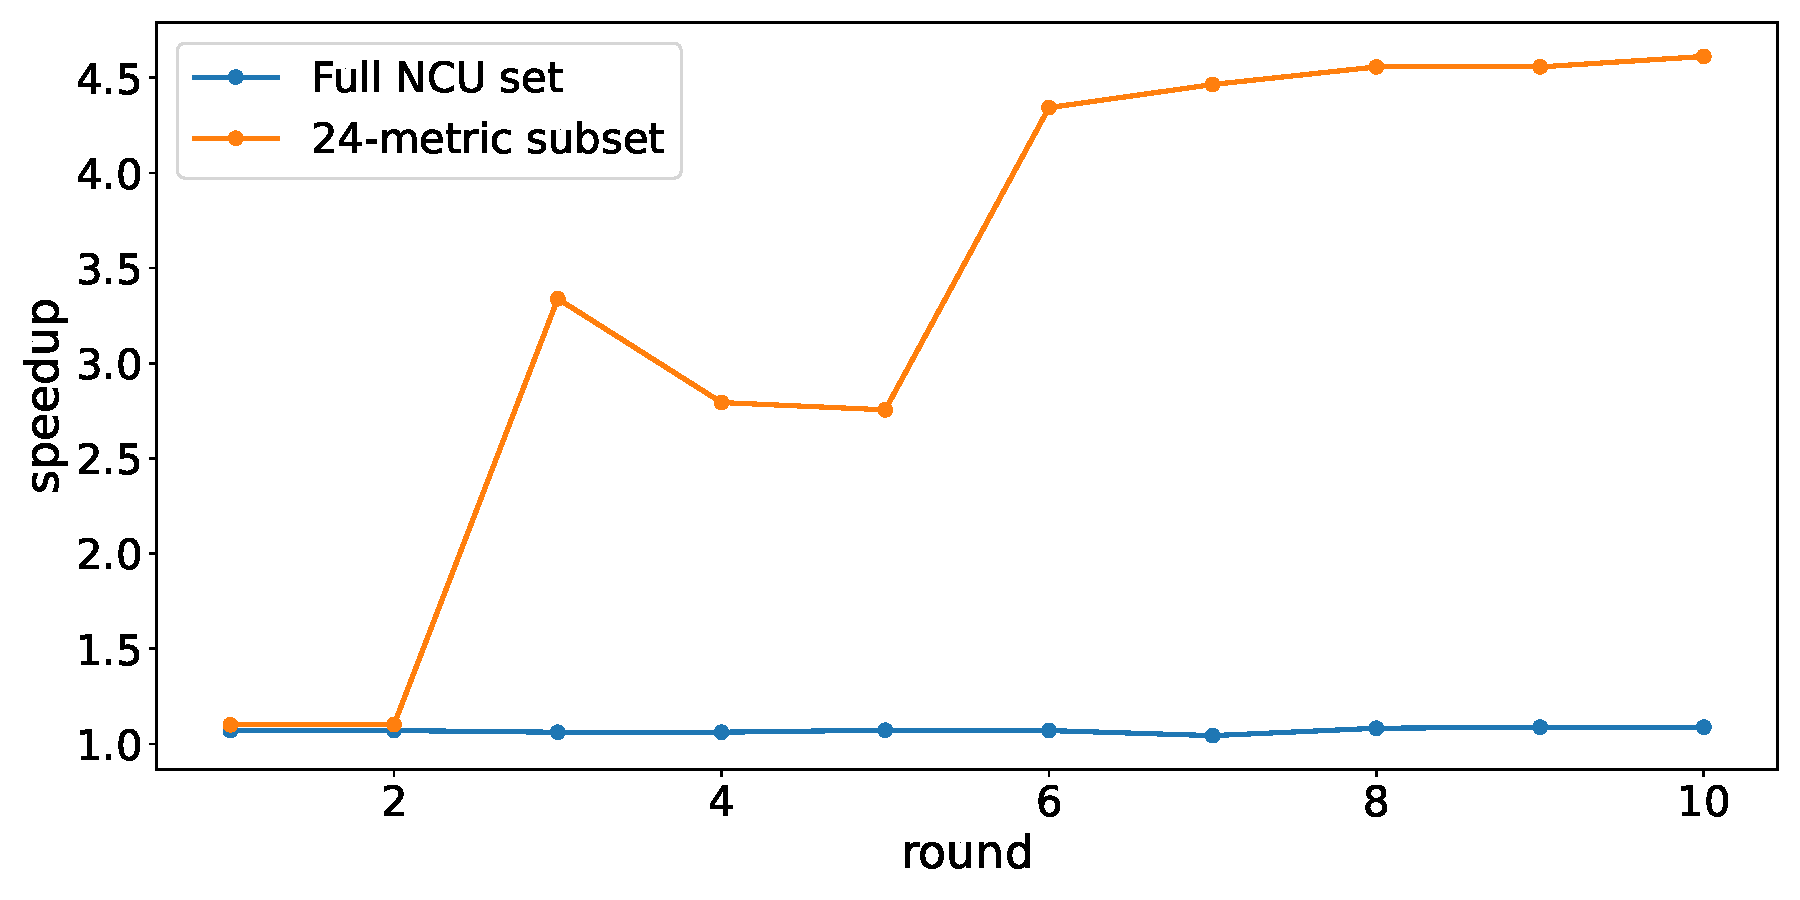
\includegraphics[width=0.8\linewidth]{pic/why_subset.pdf}
  \caption{Generated kernel performance comparison between Full-metrics input(blue line) vs. Metrics subset input(orange line) for Judge agent on Level 2 task 51. }
  \label{fig:why_subset}
\end{figure}

As shown in Figure~\ref{fig:why_subset}, we compare two configurations on a representative task. (i) The Judge agent receives {\it all} raw NCU metrics in each round and provides feedback to the Coder agent. (ii) The Judge agent receives only the 24 key metrics selected by our method and captures only 3-4 critical metrics in each round to generate optimization suggestion.

Within 10 iterative rounds, the Judge agent using full NCU metrics fails to guide the Coder agent toward better kernels. The performance of the generated kernels remains almost unchanged, despite repeated interactions. In contrast, when the Judge agent is restricted to use subset metrics, the performance of generated kernels varies across rounds and is often improved. This process eventually leads to a substantial speedup. 



In addition, we carefully reviewed how the Judge identified bottlenecks and proposed optimizations in both configurations, full set vs. 24-subset. We select one Judge's response from the optimization round to better illustrate the difference in judge output, with full NCU and with a subset of NCU as judge input.

\begin{tcolorbox}[mybox, title={Response by using the full NCU metrics set}]
\ttfamily 
\begin{verbatim}
{"bottleneck": "Long-scoreboard stalls from re-loading GEMM output out of DRAM
(gemm_out round-trip dominates cycles).",

"optimisation method": "Fuse the Linear GEMM and the current epilogue into one FP16
tensor-core CUTLASS kernel that performs subtract, row-mean, GELU and residual add
in-register, avoiding global-memory re-reads.",

"modification plan": "Write CUTLASS custom epilogue functor; use cublasLt or cutlass::
gemm_universal to compute GEMM+A, keep accumulators in registers, warp-reduce to mean,
apply GELU, add x_orig, directly store final output; expose via new PyTorch extension."}
\end{verbatim}
\normalfont
\end{tcolorbox}

\begin{tcolorbox}[redbox, title={Response by using the 24 key NCU subset}]
\ttfamily 
\begin{verbatim}
{"bottleneck": "Kernel is DRAM-bound (102.9 % peak); 57 % long-scoreboard stalls from
second pass reading original_x.",

"optimisation method": "Fuse the second loop: cache each thread’s original_x elements
in registers during diff accumulation, then add gelu_val and store, eliminating the 
extra B×F global read.",

"modification plan": "Replace two for-loops with one: load linear_out, subtract, and
original_x together, keep original_x[16] in per-thread array, finish reduction, add 
gelu_val, write to output; ~4 MB traffic per batch, >30 % speedup."}
\end{verbatim}
\normalfont
\end{tcolorbox}
Based on these two responses,we find that judge with full set NCU mertics tends to misidentify the true bottleneck.The judge with full set NCU metrics attributes the bottleneck to re-loading gemm\_out and recommends a monolithic CUTLASS epilogue that performs row-mean/GELU/residual in registers. This diagnosis is misaligned with our kernel’s access pattern and is hard to realize for general shapes due to cross-tile aggregation. In contrast, the judge with 24-key subset correctly identifies a DRAM-bound kernel dominated by the second pass over x\_orig, and proposes a one-pass rewrite that caches x\_orig in registers during the first traversal and writes back after GELU, eliminating an entire B×F global memory read. This change is lightweight, architecture-agnostic, and yields consistent speedups (e.g., about 4 MB less traffic per batch, more than 30\% in our setting).


\subsection{Top-20 NCU metrics Example}\label{app:top-20}

 This section reports, in several example tasks, the Top-20 Nsight Compute (NCU) metrics most correlated with runtime, ranked by the absolute value of the Pearson correlation coefficient. Here, runtime refers to the kernel’s execution time. When the correlation coefficient is positive, larger metric values typically imply longer execution time; when it is negative, larger metric values typically imply shorter execution time. All metric names follow their original name in NCU.



\scriptsize
\begin{longtable}{>{\raggedright\arraybackslash}p{0.63\textwidth}
                  S[table-format=+1.6]
                  S[table-format=1.6]}
\caption{Task-Conv2D: Pearson correlation with runtime (Top-20).}
\label{tab:app-conv2d-top20}\\
\toprule
\textbf{Metric Name} & {\textbf{Correlation}} & {\textbf{Abs Correlation}} \\
\midrule
\endfirsthead
\toprule
\textbf{Metric Name} & {\textbf{Correlation}} & {\textbf{Abs Correlation}} \\
\midrule
\endhead
\midrule
\multicolumn{3}{r}{\small Continued on next page} \\
\endfoot
\bottomrule
\endlastfoot

\Metric{sm\_\_cycles\_active.avg}                                  &  1.000000 & 1.000000 \\
\Metric{gpc\_\_cycles\_elapsed.max}                                &  1.000000 & 1.000000 \\
\Metric{launch\_\_occupancy\_limit\_shared\_mem}                    &  0.945507 & 0.945507 \\
\Metric{dram\_\_bytes.sum.per\_second}                              & -0.924251 & 0.924251 \\
\Metric{gpu\_\_dram\_throughput.avg.pct\_of\_peak\_sustained\_elapsed} & -0.924155 & 0.924155 \\
\Metric{smsp\_\_inst\_executed.avg}                                 &  0.916287 & 0.916287 \\
\Metric{smsp\_\_inst\_executed.sum}                                 &  0.916287 & 0.916287 \\
\Metric{smsp\_\_inst\_issued.avg}                                   &  0.916262 & 0.916262 \\
\Metric{smsp\_\_inst\_issued.sum}                                   &  0.916262 & 0.916262 \\
\Metric{lts\_\_t\_sector\_hit\_rate.pct}                            &  0.839237 & 0.839237 \\
\Metric{smsp\_\_sass\_average\_branch\_targets\_threads\_uniform.pct} &  0.810334 & 0.810334 \\
\Metric{lts\_\_throughput.avg.pct\_of\_peak\_sustained\_elapsed}    & -0.787261 & 0.787261 \\
\Metric{smsp\_\_inst\_executed\_op\_branch.sum}                     &  0.746483 & 0.746483 \\
\Metric{launch\_\_grid\_size}                                       &  0.745917 & 0.745917 \\
\Metric{l1tex\_\_t\_sector\_hit\_rate.pct}                          &  0.728356 & 0.728356 \\
\Metric{gpc\_\_cycles\_elapsed.avg.per\_second}                     &  0.728053 & 0.728053 \\
\Metric{dram\_\_cycles\_elapsed.avg.per\_second}                    &  0.665784 & 0.665784 \\
\Metric{launch\_\_waves\_per\_multiprocessor}                       &  0.627478 & 0.627478 \\
\Metric{launch\_\_thread\_count}                                    &  0.627478 & 0.627478 \\
\Metric{launch\_\_shared\_mem\_per\_block\_static}                  & -0.610501 & 0.610501 \\

\end{longtable}
% \end{landscape}
% ----- Task-B (SpMM) -----
\scriptsize
\begin{longtable}{>{\raggedright\arraybackslash}p{0.63\textwidth}
                  S[table-format=+1.6]
                  S[table-format=1.6]}
\caption{Task-SpMM: Pearson correlation with runtime (Top-20).}
\label{tab:app-spmm-top20}\\
\toprule
\textbf{Metric Name} & {\textbf{Correlation}} & {\textbf{Abs Correlation}} \\
\midrule
\endfirsthead
\toprule
\textbf{Metric Name} & {\textbf{Correlation}} & {\textbf{Abs Correlation}} \\
\midrule
\endhead
\midrule
\multicolumn{3}{r}{\small Continued on next page} \\
\endfoot
\bottomrule
\endlastfoot

\Metric{gpc\_\_cycles\_elapsed.max}                                &  0.999993 & 0.999993 \\
\Metric{sm\_\_cycles\_active.avg}                                  &  0.998432 & 0.998432 \\
\Metric{gpu\_\_compute\_memory\_request\_throughput.avg.pct\_...}  & -0.967284 & 0.967284 \\
\Metric{gpu\_\_compute\_memory\_throughput.avg.pct\_of\_peak\_...} & -0.964455 & 0.964455 \\
\Metric{lts\_\_t\_sector\_hit\_rate.pct}                           &  0.951201 & 0.951201 \\
\Metric{dram\_\_bytes.sum.per\_second}                              & -0.926134 & 0.926134 \\
\Metric{gpu\_\_dram\_throughput.avg.pct\_of\_peak\_sustained\_...} & -0.925856 & 0.925856 \\
\Metric{l1tex\_\_throughput.avg.pct\_of\_peak\_sustained\_active}  &  0.871262 & 0.871262 \\
\Metric{sm\_\_inst\_executed.avg.per\_cycle\_elapsed}              & -0.837675 & 0.837675 \\
\Metric{smsp\_\_issue\_inst0.avg.pct\_of\_peak\_sustained\_active} &  0.837284 & 0.837284 \\
\Metric{smsp\_\_issue\_active.avg.pct\_of\_peak\_sustained\_...}   & -0.837284 & 0.837284 \\
\Metric{smsp\_\_issue\_active.avg.per\_cycle\_active}              & -0.837283 & 0.837283 \\
\Metric{sm\_\_inst\_issued.avg.per\_cycle\_active}                 & -0.836185 & 0.836185 \\
\Metric{sm\_\_inst\_issued.avg.pct\_of\_peak\_sustained\_active}   & -0.836185 & 0.836185 \\
\Metric{sm\_\_inst\_executed.avg.per\_cycle\_active}               & -0.836160 & 0.836160 \\
\Metric{sm\_\_instruction\_throughput.avg.pct\_of\_peak\_sust...}  & -0.806478 & 0.806478 \\
\Metric{smsp\_\_average\_warp\_latency\_per\_inst\_issued.ratio}   &  0.802793 & 0.802793 \\
\Metric{smsp\_\_average\_warps\_active\_per\_inst\_executed.ratio} &  0.802777 & 0.802777 \\
\Metric{derived\_\_smsp\_\_inst\_executed\_op\_branch\_pct}        & -0.728768 & 0.728768 \\
\Metric{smsp\_\_warps\_eligible.avg.per\_cycle\_active}            & -0.630772 & 0.630772 \\
\end{longtable}
\normalsize
\subsection{Key Subset of 24 NCU Metrics}\label{app:key24}

The table below lists the exact 24 metrics in our NCU key subset, as a result of Algorithm~\ref{alg::alg1},~\ref{alg::alg2}

\scriptsize
\begin{longtable}{rl}
\caption{The 24-metric key subset.}
\label{tab:key24}\\
\toprule
\textbf{\#} & \textbf{Metric Name} \\
\midrule
\endfirsthead
\toprule
\textbf{\#} & \textbf{Metric Name} \\
\midrule
\endhead
\midrule
\multicolumn{2}{r}{\small Continued on next page}\\
\endfoot
\bottomrule
\endlastfoot

1  & \Metric{sm\_\_cycles\_active.avg} \\
2  & \Metric{sm\_\_warps\_active.avg.pct\_of\_peak\_sustained\_active} \\
3  & \Metric{launch\_\_occupancy\_limit\_blocks} \\
4  & \Metric{launch\_\_occupancy\_limit\_registers} \\
5  & \Metric{launch\_\_occupancy\_limit\_shared\_mem} \\
6  & \Metric{launch\_\_registers\_per\_thread} \\
7  & \Metric{sm\_\_inst\_executed.sum} \\
8  & \Metric{sm\_\_inst\_executed\_pipe\_fp32.avg.pct\_of\_peak\_sustained\_active} \\
9  & \Metric{sm\_\_inst\_executed\_pipe\_tensor.avg.pct\_of\_peak\_sustained\_active} \\
10 & \Metric{dram\_\_bytes\_read.sum} \\
11 & \Metric{dram\_\_bytes\_write.sum} \\
12 & \Metric{dram\_\_throughput.avg.pct\_of\_peak\_sustained\_elapsed} \\
13 & \Metric{dram\_\_bytes.sum.per\_second} \\
14 & \Metric{gpu\_\_dram\_throughput.avg.pct\_of\_peak\_sustained\_elapsed} \\
15 & \Metric{l1tex\_\_t\_sector\_hit\_rate.pct} \\
16 & \Metric{l1tex\_\_throughput.avg.pct\_of\_peak\_sustained\_active} \\
17 & \Metric{lts\_\_t\_sector\_hit\_rate.pct} \\
18 & \Metric{lts\_\_throughput.avg.pct\_of\_peak\_sustained\_active} \\
19 & \Metric{smsp\_\_warp\_issue\_stalled\_memory\_dependency\_per\_warp\_active.pct} \\
20 & \Metric{smsp\_\_warp\_issue\_stalled\_short\_scoreboard\_per\_warp\_active.pct} \\
21 & \Metric{smsp\_\_warp\_issue\_stalled\_long\_scoreboard\_per\_warp\_active.pct} \\
22 & \Metric{smsp\_\_warp\_issue\_stalled\_barrier\_per\_warp\_active.pct} \\
23 & \Metric{smsp\_\_warp\_issue\_stalled\_branch\_resolving\_per\_warp\_active.pct} \\
24 & \Metric{smsp\_\_sass\_average\_branch\_targets\_threads\_uniform.pct} \\
\end{longtable}
\normalsize
\section{CUDA-L1}\label{app:cuda-l1}
In our replication efforts, we found that the authors of CUDA-L1 released only the final, generated kernels for each task. After carefully studying these cases, we identified several interesting findings.

First, We found that CUDA-L1 tends to emphasize PyTorch-level optimizations rather than generating and refining custom CUDA kernels. This pattern also emerged as the most frequent issue in their provided case. Although CUDA-L1 reports the top-10 cases with the largest speedups, our review shows that nine of these ten final solutions do not use custom CUDA kernels; instead, they rely heavily on official PyTorch implementations. We show several cases of their results below.

This is the top-ranked entry in their \emph{KernelBench Tasks Ranked by RL-CUDA1 Acceleration (Top-10)}: Level 2 Task 83, with a reported $120.3\times$ speedup. It contains no CUDA kernel.
% ====== Level 2 Task 83 (blue mybox) ======
\begin{tcolorbox}[mybox, title={Level 2 Task 83 — Reported $120.3\times$ Speedup}]
\ttfamily
\begin{verbatim}
import torch
import torch.nn as nn

class ModelNew(nn.Module):
    """
    Optimized implementation of a model that performs a 3D convolution,
    applies Group Normalization, minimum, clamp, and dropout.
    
    Args:
        in_channels (int): Number of input channels
        out_channels (int): Number of output channels
        kernel_size (int or tuple): Size of the convolving kernel
        groups (int): Number of groups for GroupNorm
        min_value (float): Minimum value for clamp operation
        max_value (float): Maximum value for clamp operation
        dropout_p (float): Dropout probability
    """
    def __init__(self, in_channels, out_channels, kernel_size, groups, min_value, 
    max_value, dropout_p):
        super(ModelNew, self).__init__()
        # Store the original layers for parameter compatibility
        self.conv = nn.Conv3d(in_channels, out_channels, kernel_size)
        self.norm = nn.GroupNorm(groups, out_channels)
        self.dropout = nn.Dropout(dropout_p)
        self.min_value = min_value
        self.max_value = max_value
        self.dropout_p = dropout_p
        
        # Pre-compute convolution parameters for output shape calculation
        if isinstance(kernel_size, int):
            self.kernel_size = (kernel_size, kernel_size, kernel_size)
        else:
            self.kernel_size = kernel_size
            
        self.stride = self.conv.stride
        self.padding = self.conv.padding
        self.dilation = self.conv.dilation

    def forward(self, x):
        x = self.conv(x)
        x = self.norm(x)
        x = torch.minimum(x, torch.tensor(self.min_value, device=x.device))
        x = torch.clamp(x, min=self.min_value, max=self.max_value)
        x = self.dropout(x)
        return x

# Keep ALL hyperparameters EXACTLY as shown in the reference implementation
batch_size = 128
in_channels = 3
out_channels = 16
depth, height, width = 16, 32, 32
kernel_size = 3
groups = 8
min_value = 0.0
max_value = 1.0
dropout_p = 0.2

def get_inputs():
    return [torch.randn(batch_size, in_channels, depth, height, width)]

def get_init_inputs():
    return [in_channels, out_channels, kernel_size, groups, min_value, max_value, 
    dropout_p]
\end{verbatim}
\normalfont
\end{tcolorbox}


The second-ranked case is Level-1 Task 12 (Matmul with diagonal matrices), with a reported 64.4× speedup, which also contains no CUDA kernel:
\begin{tcolorbox}[redbox, title={Level 1 Task 12 — Reported $64.4\times$ Speedup}]
\ttfamily
\begin{verbatim}
# diag_mm_compare.py
import time
import math
import torch
import torch.nn as nn
import torch.nn.functional as F

# -------------------------------
# Reference implementation
# -------------------------------
class Model(nn.Module):
    """
    Simple model that performs a matrix multiplication of a diagonal matrix with another
    matrix.
    C = diag(A) * B
    """
    def __init__(self):
        super(Model, self).__init__()

    def forward(self, A, B):
        """
        Args:
            A (torch.Tensor): 1D tensor, diagonal entries. Shape: (N,)
            B (torch.Tensor): 2D tensor. Shape: (N, M)
        Returns:
            torch.Tensor: (N, M)
        """
        return torch.diag(A) @ B


# -------------------------------
# Optimized implementation
# -------------------------------
class ModelNew(nn.Module):
    """
    Optimized model that performs a matrix multiplication of a diagonal matrix with another
    matrix.
    C = diag(A) * B
    """
    def __init__(self):
        super(ModelNew, self).__init__()

    def forward(self, A, B):
        """
        Args:
            A (torch.Tensor): 1D tensor, diagonal entries. Shape: (N,)
            B (torch.Tensor): 2D tensor. Shape: (N, M)
        Returns:
            torch.Tensor: (N, M)
        """
        # Equivalent to torch.diag(A) @ B, but avoids forming the full diagonal matrix
        return B * A.unsqueeze(1)


# -------------------------------
# Hyperparameters & inputs
# -------------------------------
M = 4096
N = 4096

def get_inputs(device=None, dtype=torch.float32):
    A = torch.randn(N, device=device, dtype=dtype)
    B = torch.randn(N, M, device=device, dtype=dtype)
    return [A, B]

def get_init_inputs():
    return []  # No special initialization inputs needed
\end{verbatim}
\normalfont
\end{tcolorbox}
In addition, we observed many reported speedups that are effectively equal to one (clustered around 1.00, typically within ±5\%). A closer inspection shows that, in these cases, the system falls back to the original PyTorch operator when the custom kernel fails to compile, which naturally yields no measurable speedup.

For example, below is the forward method from the final solution for KernelBench Level-1 Task 3 generated by CUDA-L1. This code get from the CUDA-L1's official Github. We observe that the method first attempts to call a \emph{custom CUDA kernel}; however, upon any compilation failure or exception, it immediately falls back to \texttt{torch.bmm(A, B)}. Crucially, \texttt{torch.bmm(A, B)} is exactly the operator that this task asks to be replaced by a custom kernel, meaning the fallback undermines the task's objective. This explains why the reported speedup is only 1.006×.
\begin{tcolorbox}[mybox, title={Level 1 Task 3 — Reported $1.006\times$ Speedup}]
\ttfamily
\begin{verbatim}
    def forward(self, A: torch.Tensor, B: torch.Tensor) -> torch.Tensor:
        """
        Performs batched matrix multiplication.

        Args:
            A: Input tensor of shape (batch_size, m, k).
            B: Input tensor of shape (batch_size, k, n).

        Returns:
            C: Output tensor of shape (batch_size, m, n).
        """
        # Fall back to torch.bmm if CUDA module failed to load
        if ModelNew._cuda_module is None:
            return torch.bmm(A, B)
        
        # Check if inputs are on CUDA
        if not A.is_cuda or not B.is_cuda:
            A = A.cuda() if not A.is_cuda else A
            B = B.cuda() if not B.is_cuda else B
        
        # Ensure inputs are contiguous and float32
        A = A.contiguous().float()
        B = B.contiguous().float()
        
        # Use custom CUDA kernel
        try:
            result = ModelNew._cuda_module.batched_matmul(A, B)
            if not A.is_cuda:
                result = result.cpu()
            return result
        except Exception as e:
            print(f"Error in custom kernel: {e}, falling back to torch.bmm")
            return torch.bmm(A, B)
\end{verbatim}
\normalfont
\end{tcolorbox}

\section{Details of Benchmark}
\subsection{KernelBench}\label{KernelBench}
\textbf{KernelBench} is a standardized benchmark designed to evaluate the capability of large language models (LLMs) in CUDA kernel generation and optimization.
It consists of 270 tasks across four levels of increasing difficulty, of which Levels 1–3 (250 tasks in total) are commonly adopted for evaluation. Each task provides a PyTorch reference implementation together with fixed input–output specifications, enabling automated correctness and performance validation.

\begin{itemize}
\item \textbf{Level 1 (Basic Operators):} Contains simple, low-level operators such as matrix multiplication, element-wise operations, and reductions. These tasks primarily test the ability to generate functionally correct CUDA kernels.
\item \textbf{Level 2 (Composite Operations):} Involves multi-step operator combinations, requiring the model to compose multiple CUDA primitives and manage intermediate memory efficiently. These tasks test the capacity for more complex code synthesis.
\item \textbf{Level 3 (End-to-End Models):} Includes challenging kernels derived from full neural network architectures such as AlexNet, VGG, and ResNet components. These tasks assess the ability to produce efficient, large-scale kernels under realistic deep learning workloads.
\item \textbf{Level 4 (Optional):} The full benchmark also defines an advanced level with additional research-oriented tasks, but this is less frequently adopted due to its complexity and lack of standardized evaluation setups.
\end{itemize}

KernelBench has become a widely used benchmark in recent work on LLM-based code generation \citep{deepreinforce2025cudal1, kevin-multi-turn-rl, lange2025robustagenticcudakernel}, as it provides a controlled and reproducible environment to measure both \emph{correctness} (functional equivalence to PyTorch) and \emph{efficiency} (execution speed relative to PyTorch).
In our study, we adopt all Level 1–3 tasks, following prior work, to ensure fair comparison across baselines.



\subsection{Our stratified random subset \(\mathcal{D}^{*}\)}
\label{subset}
While our main evaluation is conducted on the full KernelBench Level 1–3 benchmark 
(250 tasks in total), we additionally construct a stratified subset $\mathcal{D}^{*}$ 
to enable detailed analysis and fair comparison, while reducing computation cost in experiments.  

The construction of $\mathcal{D}^{*}$ follows two principles:  
(1) \textbf{Coverage across difficulty levels.} Since KernelBench is stratified by 
increasing task complexity (Level~1: single-operator tasks, Level~2: multi-step fused operators, 
Level~3: full network components), we ensure that the sampled subset preserves the relative 
distribution of difficulty.  
(2) \textbf{Diversity of task types.} Within each level, we sample tasks uniformly across different 
operator categories (e.g., elementwise ops, reductions, convolutions, fused blocks) so that the 
subset remains representative of the overall benchmark.  

Concretely, we perform stratified random sampling with a fixed 10\% ratio for each level, 
resulting in a subset of 10 tasks from Level~1, 10 tasks from Level~2, and 5 tasks from Level~3, 
for a total of 25 tasks. 
For reproducibility, the exact task IDs included in $\mathcal{D}^{*}$ are:  
\begin{itemize}
    \item \textbf{Level 1 (10 tasks):} 13, 10, 16, 29, 35, 72, 7, 89, 93, 34  
    \item \textbf{Level 2 (10 tasks):} 17, 19, 40, 3, 13, 21, 38, 28, 26, 34  
    \item \textbf{Level 3 (5 tasks):} 5, 18, 32, 41, 21
\end{itemize}

